\chapter{鮮度の視覚化の実装}
\label{chap:implementation}

本章では,第\ref{chap:verification}章で検証した鮮度の表現方法を参考に,実際にブラウザで動作する拡張機能の実装について述べる.

\newpage

\section{システム概要}
\label{sec:imp_system}

本システムは Web ブラウザとして多くのシェアを持つ\footnote{\url{https://gs.statcounter.com/browser-market-share}} Google Chrome の拡張機能での実装を行った.

開発環境には関しては,TypeScript\footnote{\url{https://www.typescriptlang.org/}}, Webpack\footnote{\url{https://webpack.js.org/}} を用いている.

本システムは,Google 検索結果一覧画面に対し,各 Web サイトの公開日を取得することでそれぞれの情報の鮮度を割り出し,外見的な劣化を加える機能を持つ.

第\ref{chap:verification}章で検証した鮮度の表現方法のうち,筆者が実装可能かつ実用的だと判断した\ref{subsec:ver-tex-sheet}の表現方法を採用している.

\begin{figure}[htbp]
  \begin{minipage}{0.5\hsize}
    \begin{center}
      \fbox{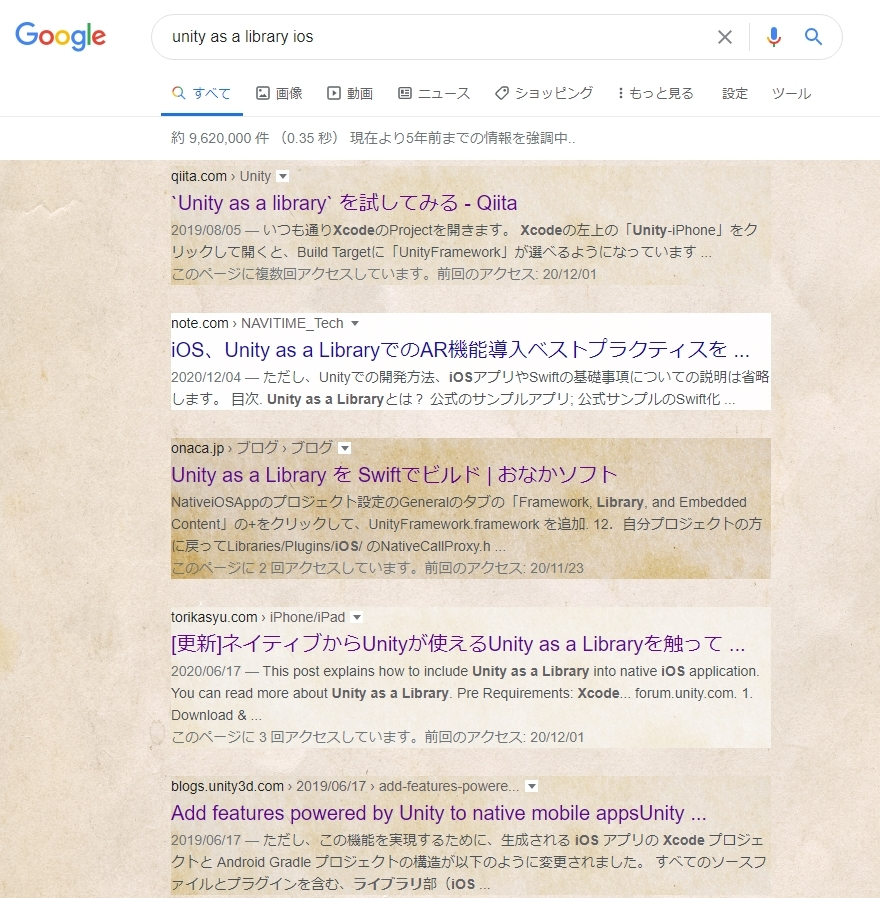
\includegraphics[width=60mm]{images/sample1.jpg}}
    \end{center}
    \caption{運用例1}
  \end{minipage}
  \begin{minipage}{0.5\hsize}
    \begin{center}
      \fbox{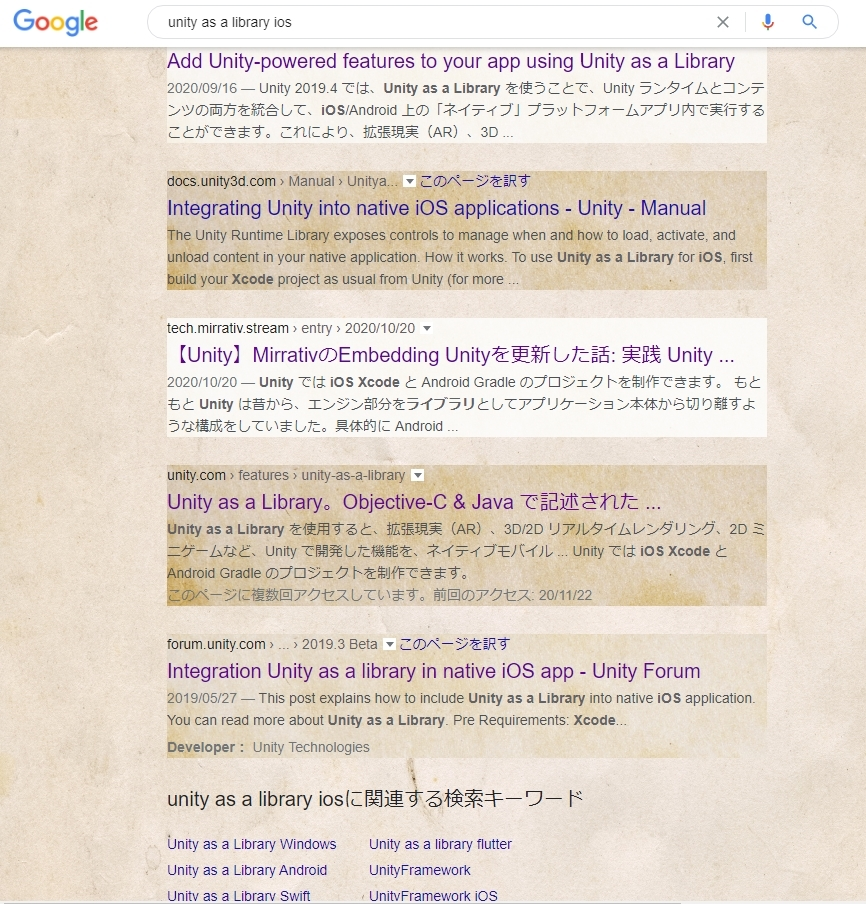
\includegraphics[width=60mm]{images/sample2.jpg}}
    \end{center}
    \caption{運用例2}
  \end{minipage}
\end{figure}

\section{鮮度の算出方法}
\label{sec:imp_calculation}

本システムでは,各情報の更新日時から現在までの経過時間(以下,時間距離とする)を参考に鮮度を算出する.算出方法として,(1)直線的なアプローチと(2)指数関数的なアプローチを考える.

以下で,二つの算出方法を実際に運用した場合の例と共に紹介するが,紹介にあたって3つの前提条件を示す.

\begin{itemize}
  \item 鮮度 $F$ は0~1の値で表し,1に近ければ近いほど新しい
  \item 時間距離 $D$ は0~1の値で表し,0に近ければ近いほど新しい
  \item 時間距離 $D$ は,情報の公開時刻 $d$ 及び現在時刻 $n$,現在時刻の5年前の時刻 $n'$ より,$ D =  (n - d) / (n - n') $ の式で算出され,結果は0以下なら0,1以上なら1として扱う\footnote{2018/01/18の情報の時間距離は,現在時刻が2021/01/24として,約 0.6 となる}
\end{itemize}

\subsubsection{直線的な算出}

$ F = 1 - D $ の式で鮮度を算出する.$D$ が大きくなるのに比例して $F$ が小さくなる.システムを運用していても特に問題はない.

\begin{figure}[htbp]
  \begin{center}
    \fbox{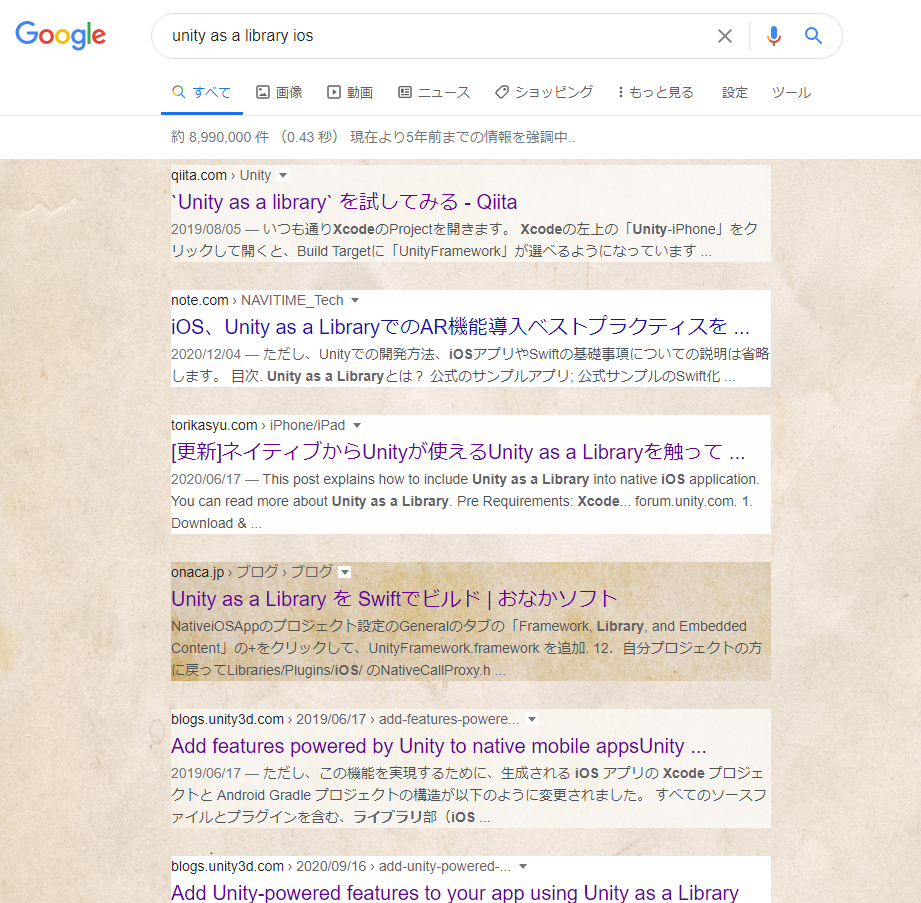
\includegraphics[width=60mm]{images/linear-sample.png}}
  \end{center}
  \caption{$ F = 1 - D $ で算出した例}
\end{figure}

\subsubsection{指数関数的な算出}

$ F =  0.01 ^ D $ の式で鮮度を算出する.$D$ の値が大きくなると $F$ が大幅に小さくなる.つまり情報が少しでも古ければ鮮度が大幅に小さくなるため,より新しい情報を強調することができる.

\begin{figure}[htbp]
  \begin{center}
    \fbox{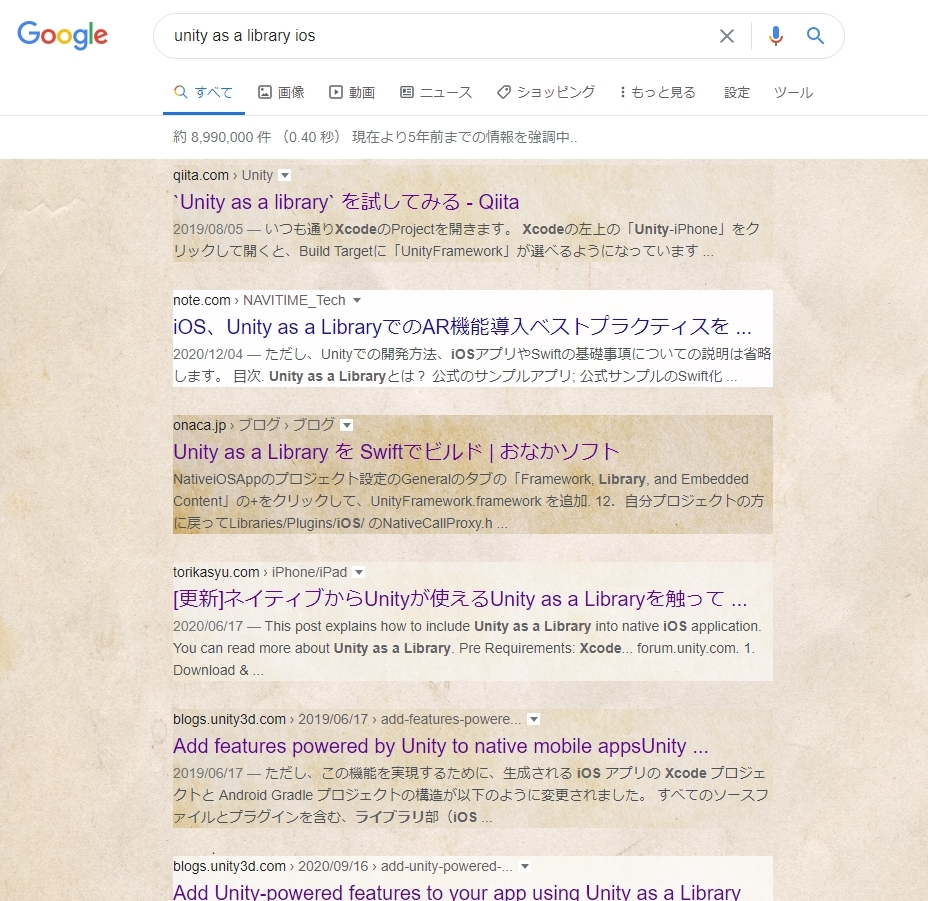
\includegraphics[width=60mm]{images/exponential-sample.png}}
  \end{center}
  \caption{$ F =  0.01 ^ D $ で算出した例}
\end{figure}

二つの算出方法を吟味した結果,指数関数的な算出方法の方が新しい情報をより強調しており,直線的な算出方法より直感的に鮮度を感じられた.

第\ref{chap:implementation}章での実装では,(2)の算出方法を利用して開発を行うこととした.
